\chapter{Résultats et expérimentations}
\label{chapitre.resultats}
	\section{Introduction}
	
	Au cours de ce chapitre, nous pésenterons dans un premier temps le schéma de contrôle en boucle fermé implémenté sur la plate-forme expérimentale.
	Ensuite de quoi nous présenterons plusieurs résultats de la loi de commande présentée en chapitre \rf{chapitre.commande}.
	Chaque expérience permettra de mettre en évidence un aspect de la loi de commande.
	
	\section{Schéma de contrôle en boucle fermée}
	\label{section.closedloop}
	
	\fig{
		\centering
		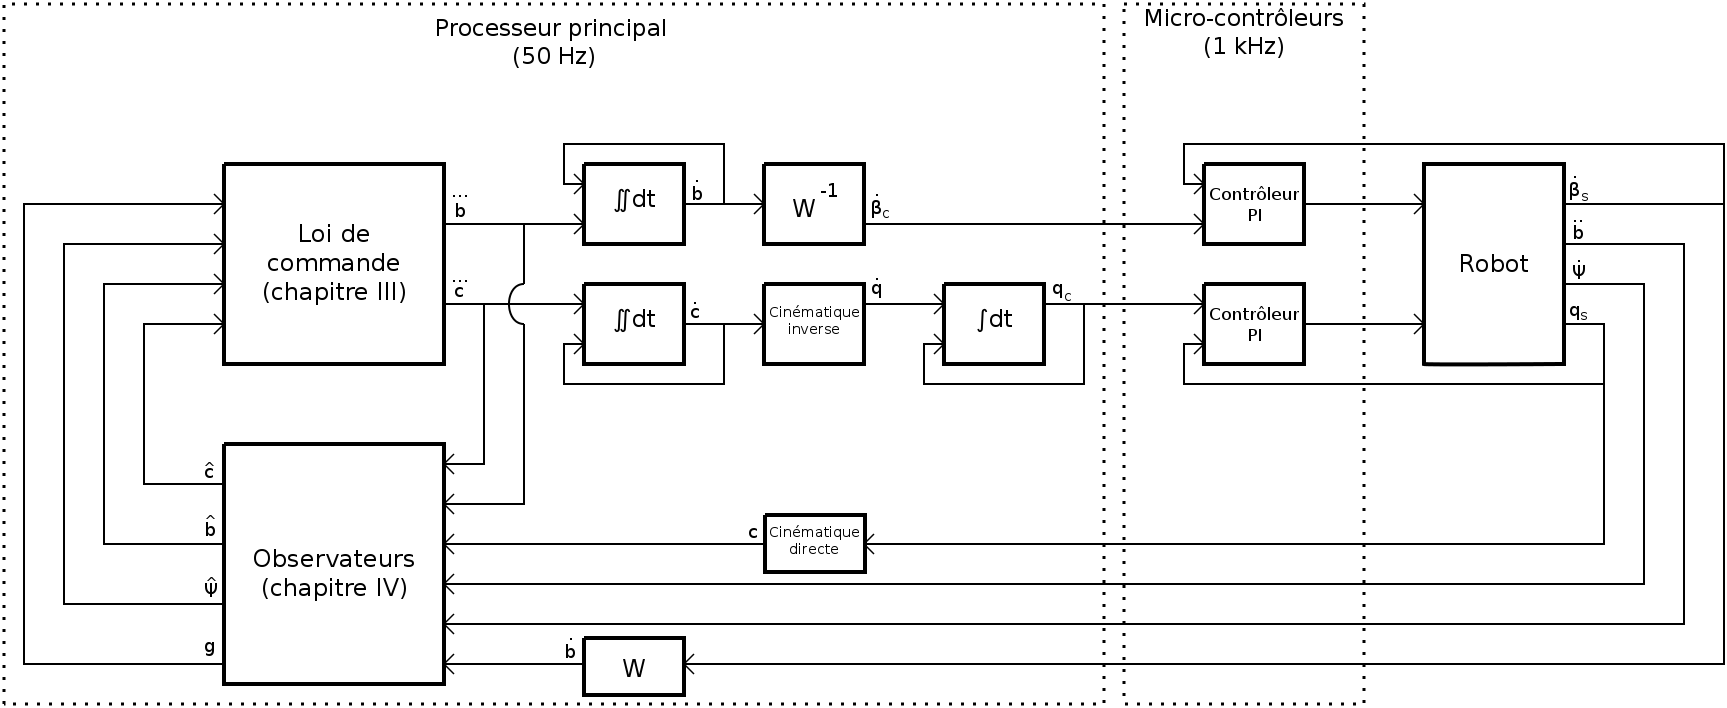
\includegraphics[width=6.5in]{closed_loop.png}
		\caption{Schéma de contrôle en boucle fermée.}
		\label{fig.closed_loop}
	}
					
	- Présenter les asservissements bas niveau (feedback)
	
	- Parler de la cinématique inverse
	
	- feedback en position de mpc
	
	- Extrapolation pour compenser le retard capteur
	
	- Stabilisation en utilisant seulement une partie de sensor
	
	- Rejeter le jeu mécanique (threshold)
	
	\section{Expériences en l'absence de perturbation et sur sol horizontal}
		\subsection{Protocole expérimental}
		
			- Trajectoire non réalisable (test de faisabilité)
			
			- Variables : jeu de pondération / nombre de masses pendule / open et close-loop mpc
			
			- Trajectoire réalisable (test de suivi)
			
			- Influence des compensations retard capteur / command sensor / jeu mécanique 
		
		\subsection{Analyse des expériences}
		
			- Intérêt du choix des pondérations
			
			- Vers une adaptation automatique des pondérations
			
			- Intérêt d'une boucle fermée plus rapide que l'échantillonage du mpc
			
			- Utilisation de deux masses au lieu d'une
			
			- Influence de la compensation du retard dans le suivi de trajectoire
			
			- Nécessité de rejeter le jeu mécanique
			
			- Dû aux bruits, ne pas utiliser entièrement sensor
		
	\section{Expériences de compensation de perturbations}
		\subsection{Protocole expérimental}
		
			- Faire basculer le robot
			
			- Variable : Durée / puissance push / direction
			
		\subsection{Analyse des expériences}
		
			- Pas de recovery quand il n'y a pas besoin
			
			- Minimisation de la vitesse d'impact (le robot peut reculer)
		
			- Pousser trop fort emmènent aux limites physique du robot
			
			- Vers une utilisation des bras pour rééquilibrer
		
		
	\section{Expériences de compensation de l'inclinaison du sol}
		\subsection{Protocole expérimental}
		
			- Faire rouler le robot préalablement sur une pente
			
			- Faire monter / descendre une pente
			
			- Modifier la direction de déplacement
			
			- Modifier la nature du sol
			
			- Push sur pente
			
			- Pente variable
		
		\subsection{Analyse des expériences}
		
			- Vitesse limitée car roues qui décolle
			
			- Problème de détection push / pente
			
			- Compensation jusqu'à 5 degrés
			
			- Problèmes de glissement au delà
			
			- Cas limite de push pendant une montée de pente
		